\documentclass{article}
\usepackage[T1]{fontenc}
\usepackage[utf8]{inputenc}
\usepackage[margin=1in]{geometry}
\usepackage{amsmath}
\usepackage{graphicx}

\newcommand{\HRule}{\rule{\linewidth}{0.5mm}}
\newcommand{\Hrule}{\rule{\linewidth}{0.3mm}}

\title{Lab Report 4}
\author{Yuhuang Chen (804449266), Zeyuan Xu (004255573)}
\date{}


\begin{document}
  \maketitle% prints the title block
  \thispagestyle{empty}
  
\section{Introduction}


\section{Theory}
The distance measure theory of this project is mainly based on a paper called \textit{Distance measuring based on stereoscopic pictures} (Mrovlje1, 2008). In this paper, the author built a mathematical model based on using two cameras to measure distance. The mathematical formulation is depicted in the picture below. 

\begin{figure}[h]
  \centering
  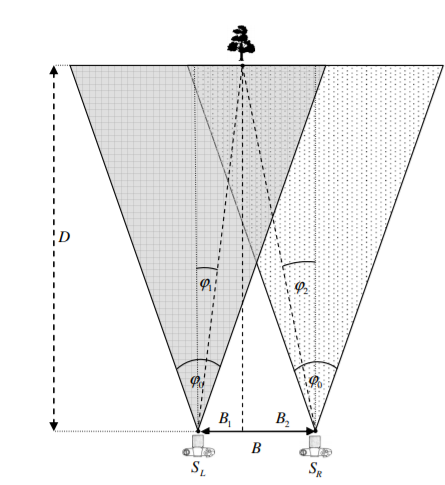
\includegraphics[width=0.5\linewidth]{theory.png}
  \caption{Mathematical Model}
  \label{fig:theory}
\end{figure}

In this picture, D is the distance between camera and the object, which is also our target. Several quantities are fixed for a specific equipment used in the measurements: $B$ is the distance between the two cameras. $\phi$ specifies the range (in degrees) of vision a camera has: in our case, it is formulated as the range of pixels. The measurement for this range is around 73 degrees. Another constant is the range of view for the two cameras combined, and we represent it as $x_0$. The formula for computing the distance is given as: 
\begin{equation}
D = \frac{B x_0}{2\tan(\frac{\phi}{2})\Delta x}
\end{equation} 
Where $\Delta x$ represents the distance between the same object in two different cameras in pixels. 

\section{Algorithms and Structure of Project}

\section{Feature Representation}

\section{Cost Function}
One key point of the project is to capture the same object on another camera: since we fixed the camera and the object on the left camera, we need to find the same object on the right camera as well. Therefore, we need metrics to determine whether a 64x64 pixel matrix on the right-hand-side is the same as the already specified pixel matrix on the left hand side. \\
The two metrics to tested on are L-1 norm and L-2 norms. In L-1 norm formulation, we define the cost to be the sum of absolute difference between every pixel in the two matrices, and this is defined as:
\begin{equation}
 \sum\limits_{1\leq i \leq 64, 1 \leq j \leq 64} |Y_{ij} - X_{ij} |
\end{equation}
This formulation defines $Y_{ij}$ as the target matrix on the right camera, its value should be a pixel value. $X_{ij}$ are fixed and are pixel values of the left camera image.\\
The L-2 norm representation of cost would be: \begin{equation}
\sum\limits_{1\leq i \leq 64, 1 \leq j \leq 64} (Y_{ij} - X_{ij})^2
\end{equation} 
Both cost functions are tested, and the better performing one (and the one we used for this project) is the L-1 norm cost function. 


\subsection{Cost Function and Feature Bagging}


\section{Summary}

\end{document}